\begin{table}
\begin{center}
\begin{tabular}{|c|}
\hline
\begin{large} PI\_PF\_OD\_100\_39SecHA1HstICent \end{large}\\
\hline
Sección central en hastial izquierdo. Armadura vertical.\\
\hline
\begin{tabular}{c|l}
\begin{minipage}{85mm}
\vspace{2mm}
\begin{center}
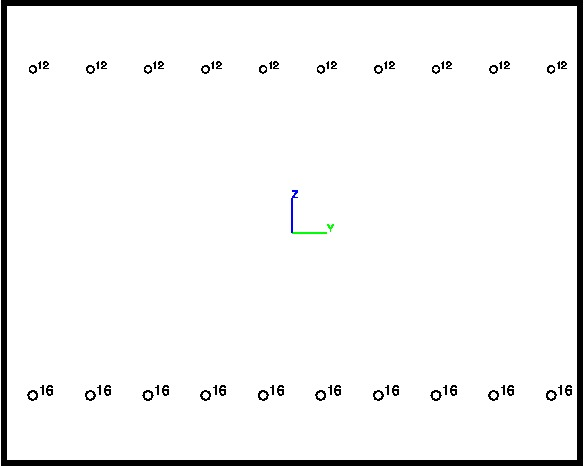
\includegraphics[width=80mm]{materials/figures/hsticentDatosScc1}
\end{center}
\vspace{1pt}
\end{minipage} & 
\begin{tabular}{l}
width: \\
$b= 1.00\ m$\\
depth: \\
$h= 0.70\ m$\\
\end{tabular} \\
\end{tabular} \\
\hline
\textbf{Materiales}:\\
\hline
\begin{tabular}{ll}
Hormigón: HA30 & Módulo de deformación longitudinal: $E_c= 28.58\ GPa$\\
\hline
Acero: B500S & Módulo elástico: $E_s= 200.00\ GPa$\\
\end{tabular} \\
\hline
\textbf{Valores estáticos}:\\
\hline
Sección bruta:\\
\hline
\begin{tabular}{ll}
$A_{bruta}= 0.700\ m^2$ & \multirow{3}{*}{Tensor de inercia ($cm^4$): $ \left( \begin{array}{ccc}647.78 & 0.00 & 0.00 \\ 0.00 & 285.83 & -0.00 \\ 0.00 & -0.00 & 583.33 \end{array} \right)$} \\
& \\
C.D.G.: $( 0.00, 0.00)\ m$  & \\
\end{tabular} \\
\hline
Sección homogeneizada:\\
\hline
\begin{tabular}{ll}
$A_{homog.}= 0.737\ m^2$ & \multirow{3}{*}{Tensor de inercia ($cm^4$): $ \left( \begin{array}{ccc}647.78 & 0.00 & 0.00 \\ 0.00 & 315.25 & -0.00 \\ 0.00 & -0.00 & 613.81 \end{array} \right)$} \\
& \\
C.D.G.: $( 0.00,-0.00)\ m$  & \\
\end{tabular} \\
\hline
\textbf{Armadura pasiva}:\\
\hline
\begin{tabular}{ll}
Área total $A_s=31.40\ cm^2$ & Cuantía geométrica $\rho= 4.49\permil$\\
\end{tabular} \\
\hline
Familias de armadura principal:\\
\hline
\begin{tabular}{cccccccc}
Id & n. barras & $\phi$ & área & c. geom. & cover. mec. & $y_{cdg}$ & $z_{cdg}$\\
 &  & $(mm)$ & $(cm^2)$ & $(\permil)$ & $(cm)$ & $(m)$ & $(m)$\\
\hline
neg & 10 & 16 & 20.10 & 2.87 &  5.0 & 0.000 & -0.282\\
\hline
pos & 10 & 12 & 11.30 & 1.61 &  5.0 & 0.000 & 0.284\\
\end{tabular} \\
\hline
Familias de armadura de cortante:\\
\hline
\begin{tabular}{cccccccc}
Id & n. ramas & $\phi$ & área & sep. & area/m & $\alpha$ & $\beta$\\
 &  & $(mm)$ & $(cm^2)$ & $(cm)$ & $(cm^2/m)$ & $( \degree)$ & $( \degree)$\\
\hline
Vz & 0 & 0 &  0.00 & 20.0 &  0.00 & 90.0 & 45.0\\
\hline
Vy & 0 & 0 &  0.00 & 20.0 &  0.00 & 90.0 & 45.0\\
\end{tabular} \\
\hline
\end{tabular}
\end{center}
\caption{Sección central en hastial izquierdo. Armadura vertical. (PI\_PF\_OD\_100\_39SecHA1HstICent).} \label{informSec}
\end{table}
